\chapter{Descripción de la máquina virtual}

En esta parte se describe con más detalle lo que se utilizo para la máquina virtual y su manejo de memoria

\section{Equipo de cómputo, lenguaje y utilerías especiales usadas}

Una PC con Windows 10, se utilizó el lenguaje de programación Python 3.10 con apoyo de las librerías de \emph{PLY, Numpy, re, json, SciPy y Matplotlib}.

La máquina virtual utiliza las librerías de emph{JSON, SciPy, NumPy y Matplotlib}. Utiliza la librería de \emph{JSON} para leer el archivo generado por el compilador y con toda la información del archivo va ejecutando el código intermedio generado por el compilador. Cuando la máquina lee una función especial utiliza las librerías de \emph{SciPy, NumPy y Matplotlib} para ejecutar dichas funciones.


\section{Descripción del proceso de Administración de Memoria en ejecución}
Para lograr ejecutar de manera correcta el código compilado es importante poder representar y manejar el espacio de memoria en la máquina virtual, de manera en la que se pueda convertir las direcciones virtuales asignadas por el compilador a espacios de memoria en la máquina.

\subsection{La Clase Memoria}

Para manejar la memoria en la máquina virtual se desarrollo la clase Memory, la cual representa un conjunto de espacios de memoria para enteros, flotantes, caracteres, booleanos y apuntadores como cinco listas. Esta clase recibe un número representando la cantidad de espacios para cada tipo de variable en su constructor y se genera una lista con el tamaño apropiado.

%Diagrama de clase de Memory
\begin{figure}[htbp]
    \centering
    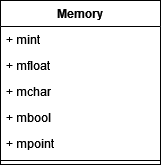
\includegraphics[scale=0.6]{chapters/chapter4/figures/Class_Memeory.png}
    \caption{Diagrama de Clase de Memory}
    \label{fig:my_label}
\end{figure}
\FloatBarrier
De esta manera se puede mapear la memoria de la máquina virtual, las listas que contienen la información, a las direcciones virtuales del compilador realizando la siguiente formula.
$$Espacio\_en\_el\_arreglo = Dir\_Virtual - Dir\_Virtual\_Base\_del\_tipo$$
Con esta formula se puede sacar la posición en el arreglo se encuentra el valor de la variable.


\subsection{Manejo de memoria global, local y temporal}

Ahora para representar el espacio de memoria en la máquina virtual se necesita primero plantear el como se debe de manejar los scopes de las variables. Para manejar las variables globales basta con crear una instancia de Memory para representarlas, pero se empieza a complicar la situación cuando se intenta representar el scope de la función principal o de cualquier otra función. Esto se debe a que Memory solo cuenta con un conjunto de arreglos, pero estos espacios de memoria cuentan no solo con variables locales sino que también con variables temporales. Para lidiar con este problema el espacio de memoria de una función se representa por un vector con dos instancias de Memory. La primera representando las variables locales y la segunda representando las variables temporales.
% imagen representando esto

\begin{figure}
    \centering
    \begin{lstlisting}[language=Python]
        globalMem = Memory(1,6,0,3)
        # El primero representa el local y el segundo el temporal
        principalMem = [Memory(1,6,0,3), Memory(7,6,0,8)] 
    \end{lstlisting}
    \caption{Representación en código de las memorias}
    \label{fig:my_label}
\end{figure}
\FloatBarrier

Con este vector ahora ya se puede manejar todos los posibles scopes de la memoria.


\subsection{El stack de memorias}

Habiendo resuelto el problema de las variables temporales y locales, surge un nuevo problema. ¿Cómo se sabe en qué memoria se está trabajando actualmente? Para resolver esto se implemento una pila, la cual maneja el contexto actual con el que se esta trabajando. La idea de usar una pila viene a la naturaleza del uso de espacios de memoria cuando se llama a una función. 
Lógicamente si seguimos el algoritmo que generan los cuádruplos, la máquina virtual va a parar la ejecución del código actual y va a saltar a realizar el código de la función. Después de acabar la función la máquina debe de regresar a donde estaba y continuar el código. Esto se podría resolver con una variable auxiliar, pero surge un problema si se utiliza una variable auxiliar cuando una función llama a otra función. 
% ejemplo con listings

\begin{figure}[htbp]
    \centering
    \begin{lstlisting}[language = Python]
        # Se llama funcion 1
        auxMem = principalMem
        .........
        # Se llama funcion 2
        auxMem = funcMem
        # Ya se perido la memoria de principal 
    \end{lstlisting}
    \caption{Representación de el uso de una variable auxiliar}
    \label{fig:my_label}
\end{figure}
\FloatBarrier
Si solo se usa una variable auxiliar la nueva función va a causar que la memoria de la función que se anda ejecutando sobre escriba a la memoria que la llamo. Pero este problema se puede resolver con una pila. Si una función llama a otra función en su ejecución lo que se puede hacer es ir guardando las memorias en la pila y cuando se dejen de utilizar se remueven del tope de la pila y se continúa utilizando el siguiente elemento en la pila. De esta manera se resuelve el problema de cuando una función llama a otra función.
\begin{figure}[htbp]
    \centering
    \begin{lstlisting}[language = Python]
        # Se llama funcion 1
        auxMem.append(principalMem)
        .........
        # Se llama funcion 2
        auxMem.append(funcMem)
        # Ahora solo se tiene que hacer pop al stack para obtener el contexto pasado
    \end{lstlisting}
    \caption{Representación de el uso de una pila para el manejo de memoria}
    \label{fig:my_label}
\end{figure}
\FloatBarrier
Esta solución no solo aplica para las funciones que son dependientes a otras, sino que también soluciona el problema de el manejo de memorias en funciones recursivas.

% ejemplo con tabla
\begin{table}[htbp]
    \centering
    \begin{tabular}{c|c c c c}
       
        Pila de Memorias & MemPrincipal & MemFuncRec & MemFuncRec & ..... \\
         
    \end{tabular}
    \caption{Representación de la pila en llamadas recursivas}
    \label{tab:my_label}
\end{table}

\section{Constantes}

Para el manejo de constantes en la memoria de la máquina virtual no fue necesario crear un espacio de memoria con la clase Memory. Para reducir la cantidad de instancias generadas se opto por pasar la tabla de constantes de compilación al archivo obj que resulta del proceso. De esta manera se puede recuperar esta información cuando se lee el archivo.  Esta información es guardada en un diccionario que puede ser accesado con la dirección virtual como la llave y nos ahorra el calculo de obtener la posición que debería de tener en memoria.